\documentclass[11pt]{article}

\usepackage[margin=1in]{geometry}
\usepackage[utf8]{inputenc}
\usepackage[T1]{fontenc}
\usepackage{lmodern}
\usepackage{amsmath}
\usepackage{graphicx}
\usepackage{booktabs}
\usepackage{float}
\usepackage{caption}
\usepackage{hyperref}

\graphicspath{{../figures/}}

\title{Project 2 Report: Fitbit Fitness Tracker Data}
\author{Lukas Anell}
\date{November 2026}

\begin{document}
\maketitle

\section*{Summary}

\section*{Introduction}

\section{Distributions and Outliers}
\label{sec:s1}

\subsection*{1(a) Heart Rate}

\begin{figure}[H]
	\centering
	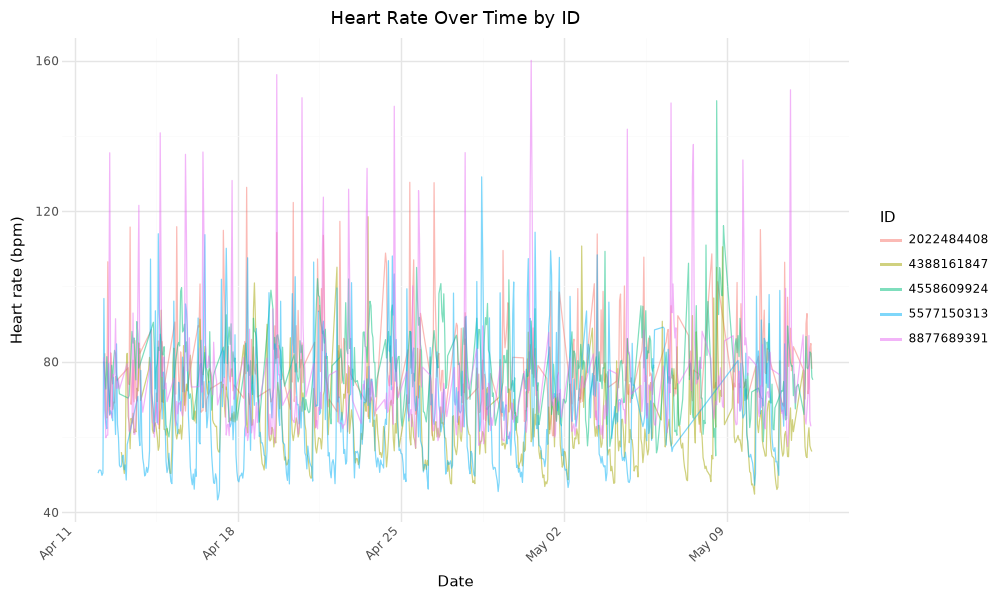
\includegraphics[width=\linewidth]{heart_rate_by_id.png}
	\caption{Hourly mean heart rate over time for five users.}
	\label{fig:heart_rate}
\end{figure}

\subsection*{1(b) Minutes Asleep}

\begin{figure}[H]
	\centering
	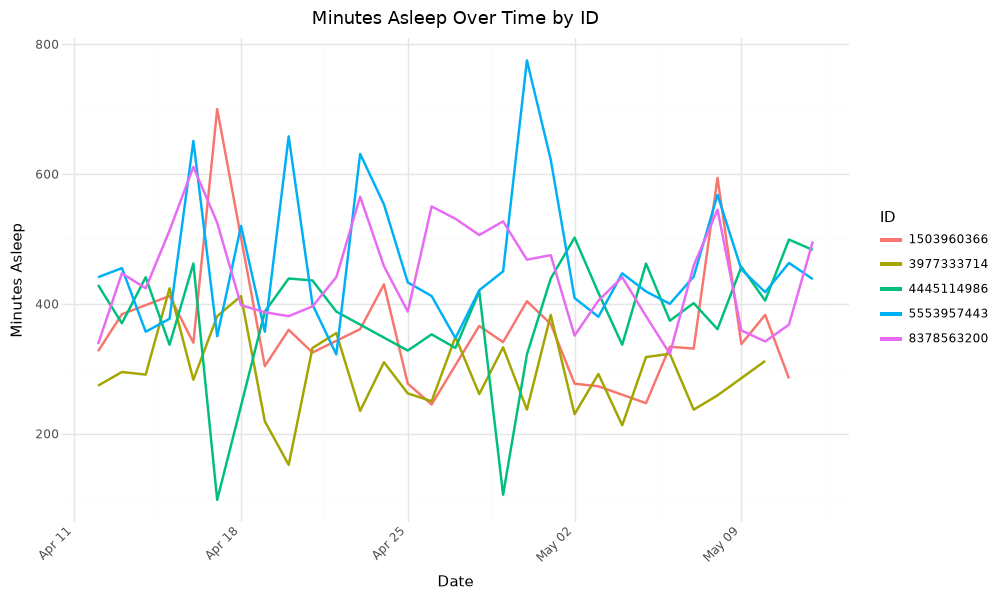
\includegraphics[width=\linewidth]{minutes_asleep_by_id.png}
	\caption{Minutes asleep over time for five users.}
	\label{fig:minutes_asleep}
\end{figure}

\subsection*{1(c) Total Steps}

\begin{figure}[H]
	\centering
	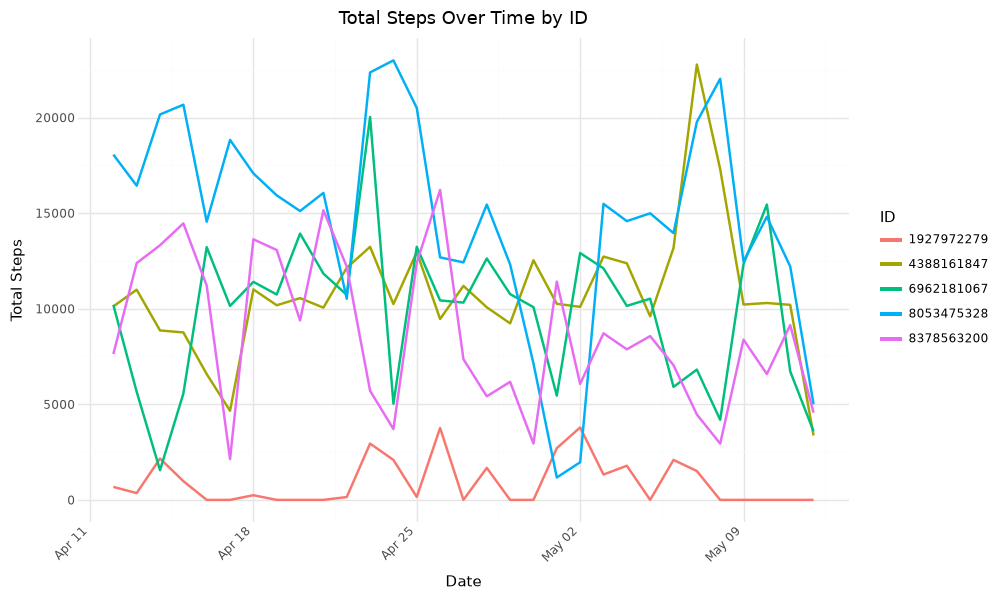
\includegraphics[width=\linewidth]{total_steps_by_id.png}
	\caption{Total steps per day over time for five users.}
	\label{fig:total_steps}
\end{figure}

\subsection*{1(d) Weight}

\begin{figure}[H]
	\centering
	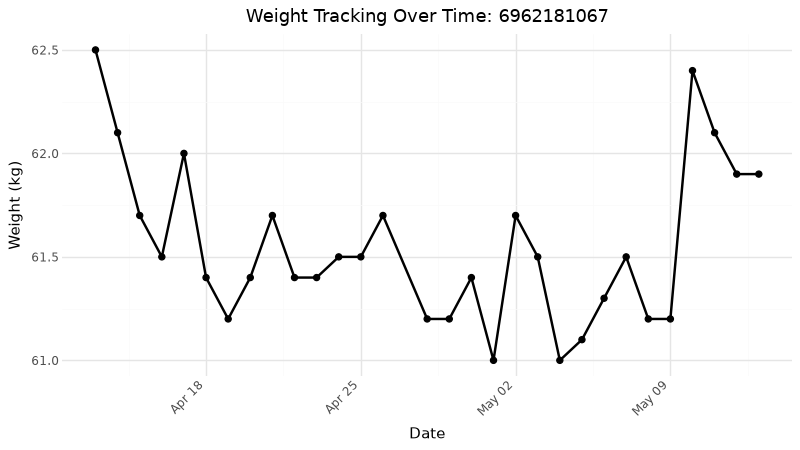
\includegraphics[width=\linewidth]{weightKb_by_date.png}
	\caption{Weight over time for the user with the most records.}
	\label{fig:weight}
\end{figure}

\section{Data Processing}
\label{sec:s2}

\subsection{Hourly and Minutely Data}

To build the hourly dataframe, I merged \texttt{hourlySteps}, \texttt{hourlyIntensities}, and \texttt{hourlyCalories} on the user \texttt{Id} and the datetime of each reading.
Similarly, the minutely dataframe merges \texttt{minuteCaloriesNarrow}, \texttt{minuteIntensitiesNarrow}, and \texttt{minuteMETsNarrow}.
I used outer merges and also checked that each merged dataframe was one-to-one, so that a duplicate key would raise an error.
In terms of shape, the hourly dataframe has 22,099 rows and 33 users, and the minutely dataframe has 1,325,580 rows and the same set of 33 users.
Neither dataframe has missing values.

The time columns were stored as 12-hour strings like \texttt{4/12/2016 12:00:00 AM}, so I converted them with an explicit format and put them into a new column named \texttt{Date}.
I did the same for \texttt{dailyActivity} and \texttt{sleepDay}.
I checked that the conversion worked by confirming that the dates only fall in April and May 2016, that all 24 hours appear, and that 12:00 AM and 12:00 PM were read correctly.
After creating \texttt{Date}, I chose to drop each dataframe's respective date column (\texttt{ActivityHour}, \texttt{ActivityDate}, \texttt{SleepDay}, etc.)

{\footnotesize
		\begin{verbatim}
Hourly (only 00:00 and 12:00 rows):
            Id  Calories                Date  TotalIntensity  AverageIntensity  StepTotal
0   1503960366        81 2016-04-12 00:00:00              20          0.333333        373
12  1503960366        73 2016-04-12 12:00:00              11          0.183333        253
24  1503960366        69 2016-04-13 00:00:00              14          0.233333        144
36  1503960366        82 2016-04-13 12:00:00              15          0.250000        486

Minutely:
           Id  Calories                Date  Intensity  METs
0  1503960366    0.7865 2016-04-12 00:00:00          0    10
1  1503960366    0.7865 2016-04-12 00:01:00          0    10
2  1503960366    0.7865 2016-04-12 00:02:00          0    10
3  1503960366    0.7865 2016-04-12 00:03:00          0    10

dailyActivity (selected columns):
           Id  TotalSteps  LightlyActiveMinutes  SedentaryMinutes  Calories       Date
0  1503960366       13162                   328               728      1985 2016-04-12
1  1503960366       10735                   217               776      1797 2016-04-13
2  1503960366       10460                   181              1218      1776 2016-04-14
3  1503960366        9762                   209               726      1745 2016-04-15

sleepDay (413 rows, before removing duplicates):
           Id  TotalSleepRecords  TotalMinutesAsleep  TotalTimeInBed       Date
0  1503960366                  1                 327             346 2016-04-12
1  1503960366                  2                 384             407 2016-04-13
2  1503960366                  1                 412             442 2016-04-15
3  1503960366                  2                 340             367 2016-04-16
\end{verbatim}
	}

\texttt{sleepDay} contains three exact duplicate rows, which I removed in Section 1(b) and wherever else I used it, so that those days weren't counted twice.

\subsection{Heart Rate}

The heart rate file has a new reading about every five seconds, so I rounded each timestamp down to the minute and took the mean of each minute's readings to get the average heart rate per minute.
This left me with 333,420 rows for 14 users.
I stored the result in its own dataframe instead of adding it to the minutely dataframe, because only 14 out of the 33 users have heart rate data, and the heart rate data only runs until 16:20 on May 12th, while the minutely data ends at 15:59.
Storing heart rate data in its own dataframe avoided dropping heartrate minutes after 15:59 or adding missing values to other columns.

	{\footnotesize
		\begin{verbatim}
             Id                Date      Value
275  2022484408 2016-04-12 12:00:00  69.272727
276  2022484408 2016-04-12 12:01:00  59.375000
277  2022484408 2016-04-12 12:02:00  59.333333
278  2022484408 2016-04-12 12:03:00  62.166667
\end{verbatim}
	}

\section{Correlation and Plots}
\label{sec:s3}

\subsection{Calories vs.\ Steps and Intensity}

\begin{figure}[H]
	\centering
	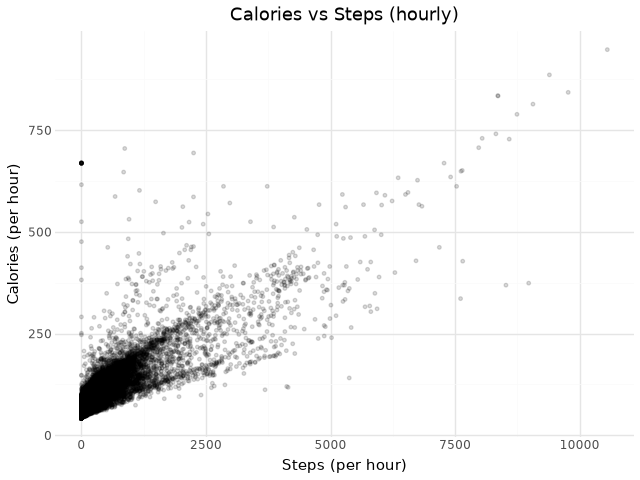
\includegraphics[width=0.8\linewidth]{calories_vs_steps.png}
	\caption{Calories per hour vs.\ steps per hour.}
	\label{fig:cal_steps}
\end{figure}

\begin{figure}[H]
	\centering
	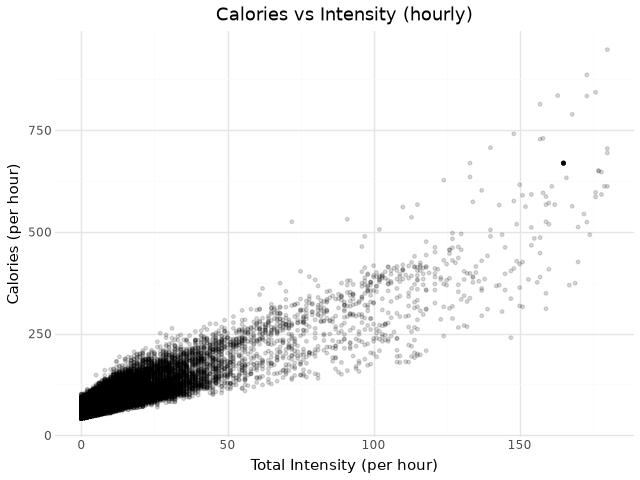
\includegraphics[width=0.8\linewidth]{calories_vs_intensity.png}
	\caption{Calories per hour vs.\ total intensity per hour.}
	\label{fig:cal_intensity}
\end{figure}

\subsection{Minutes Asleep vs.\ Time in Bed}

\begin{figure}[H]
	\centering
	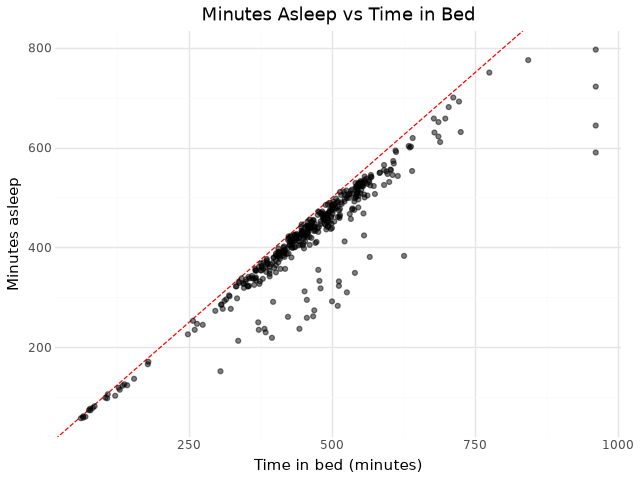
\includegraphics[width=0.8\linewidth]{asleep_vs_in_bed.png}
	\caption{Minutes asleep vs.\ time in bed (dashed line: $y = x$).}
	\label{fig:asleep_bed}
\end{figure}

\subsection{Intensity over the Day}

\begin{figure}[H]
	\centering
	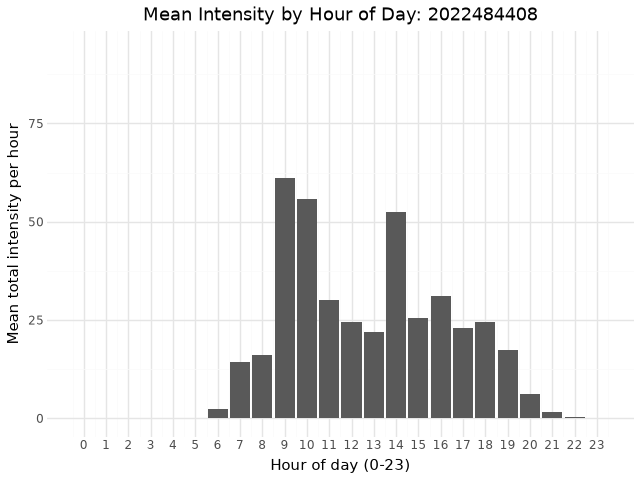
\includegraphics[width=0.7\linewidth]{intensity_by_hour_2022484408.png}
	\caption{Mean total intensity by hour of day, user 2022484408.}
	\label{fig:hour_a}
\end{figure}

\begin{figure}[H]
	\centering
	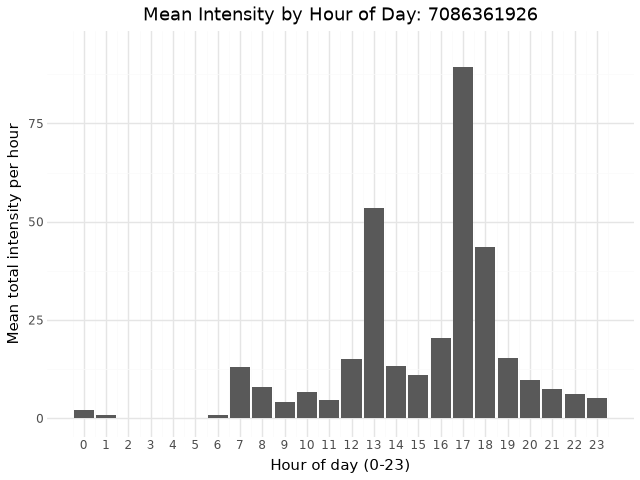
\includegraphics[width=0.7\linewidth]{intensity_by_hour_7086361926.png}
	\caption{Mean total intensity by hour of day, user 7086361926.}
	\label{fig:hour_b}
\end{figure}

\begin{figure}[H]
	\centering
	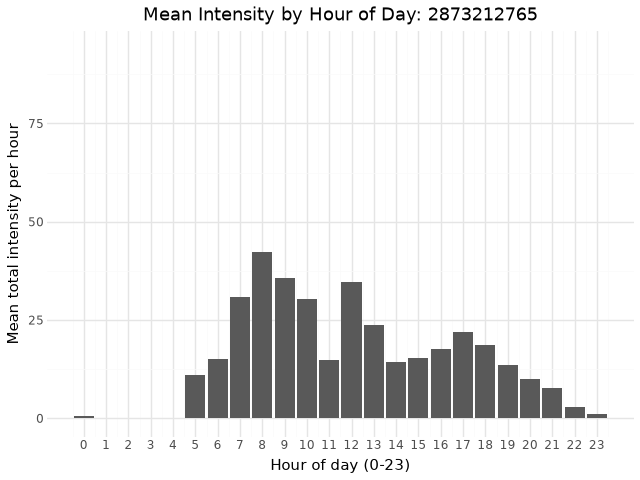
\includegraphics[width=0.7\linewidth]{intensity_by_hour_2873212765.png}
	\caption{Mean total intensity by hour of day, user 2873212765.}
	\label{fig:hour_c}
\end{figure}

\subsection{Minutes Asleep vs.\ Sedentary Minutes}

\begin{figure}[H]
	\centering
	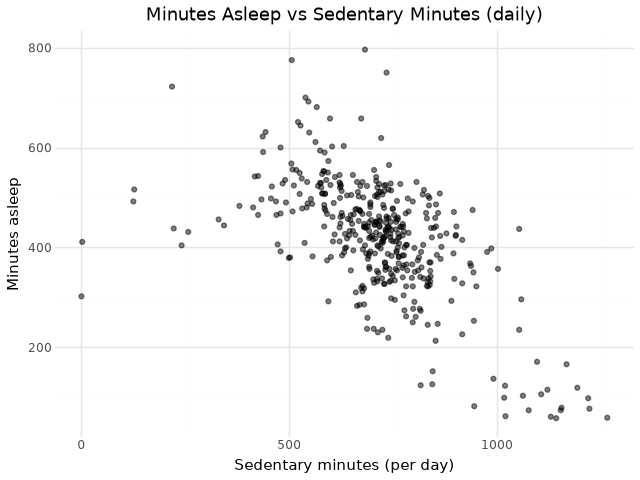
\includegraphics[width=0.8\linewidth]{asleep_vs_sedentary.png}
	\caption{Minutes asleep vs.\ sedentary minutes per day.}
	\label{fig:asleep_sed}
\end{figure}

\section{T-tests}
\label{sec:s4}

\section*{Conclusion}

\section{Reflection}
\label{sec:reflection}

\subsection{Something I Understand Differently Now}

While working on 3.4, I expected SedentaryMinutes to include the time recorded in TotalMinutesAsleep.
That would have meant they would have a positive relationship, where more sleep would go with more sedentary minutes.
Instead, the two had a correlation of $r = -0.60$.
To figure out why, I checked whether the sedentary, lightly active, fairly active, and very active minutes added up to the 1,440 minutes in a day on days with a sleep record, and it didn't add up once out of 410 days.
The leftover minutes, which was calculated as 1,440 minus the sum of the four columns, had a median of 457, which was close to the median of 432.5 minutes asleep, and they had a correlation with minutes asleep at $r = 0.63$.
This suggests that the tracker mostly leaves sleep out of sedentary time.
A day always has 1,440 minutes, so more sleep leaves fewer minutes awake that can count as sedentary, and the negative sign is largely built into how the minutes are counted, rather than showing that sitting more negatively affects sleep.
I can't confirm the tracker's exact rule based on the data, but now I understand that what a column measures depends on how the device defines it, not only what it's called.

\subsection{A Decision I Made}

When working with intensity in 3.1, I wasn't sure whether to use TotalIntensity or AverageIntensity from the hourly data.
I thought that they might be the same measurement but on different scales, so I checked the data.
\texttt{np.allclose} comparing AverageIntensity with TotalIntensity / 60 returned False, but the largest difference between them was only about $3.3 \times 10^{-7}$, which is something I'd expect if the values of AverageIntensity are rounded to six decimals.
So the False most likely came from rounding and not from a real difference.
The check returned True when using a tolerance of $10^{-6}$.
Both columns also had the same correlation with calories ($r = 0.8966$) and gave the same scatterplot shape.
Because they gave identical results, I chose to use TotalIntensity because it's an hourly total like steps and calories, which makes the plots easier to compare.

\subsection{A Moment of Uncertainty}

When plotting calories against steps and against intensity, I noticed that there was one especially dark point at 0 steps and about 670 calories in the steps plot, and it appeared at an intensity of around 165 out of 180 in the intensity plot.
My first interpretation was that it might be exercise that just doesn't register as steps, such as cycling or rowing.
But the point was solid black even though I had set the transparency to 0.15, so it couldn't just be a single observation.
I filtered for rows with 0 steps and over 600 calories, and I found that there were 16 rows that were all from one user, and all in the 05:00 hour on different days, with 15 of them having exactly the same values (669 calories and 165 intensity).
It would be very unlikely for real exercise to produce exactly identical values on 15 different mornings, so I think it's more likely that there was a recording error or some other artifact, but I can't confirm the cause just from looking at the data.
By removing the 16 rows, the correlation for steps changed from 0.815 to 0.846, and from 0.897 to 0.893 for intensity, so my conclusion that intensity is the better predictor actually didn't depend on them.

\subsection{Looking Back}

If I did this again, I would start by checking every file for repeated or duplicate rows and suspicious maximum values, before interpreting any outliers.
The 16 identical rows in 3.1 and the four nights with exactly 961 minutes in bed, which was a maximum in the dataset and from 2 different users, both looked like interesting findings when I first noticed them.
I spent a long time trying to explain them before deciding to examine the data behind them.
When inspecting the sleep data, I did find three exact duplicate rows, which kept me from double counting them.
Next time, I would just write a short script that prints the most common repeated rows and each column's maximum for every file before making any plots.

\end{document}
